\documentclass[12pt, a4paper]{article}
\usepackage[margin=0.5in]{geometry}

\usepackage{color}
\usepackage[dvipsnames]{xcolor}
\usepackage{hyperref}
\hypersetup{
    colorlinks=true,
    linkcolor=blue,
    urlcolor=blue,
    linktoc=all
}


\usepackage{amsmath}
\usepackage{mathtools}
\usepackage{amssymb}
\usepackage{cancel}
\usepackage{bm}
\usepackage{dsfont}
\usepackage{graphicx}
\usepackage{graphics}
\usepackage{xfrac}
\usepackage{array}
\setcounter{MaxMatrixCols}{40}

\usepackage{enumerate}
\usepackage{enumitem}
\usepackage{multirow}

%inclusions carried over from past class homework formats
\usepackage{units}
\usepackage{fullpage}
\usepackage{alltt}
\usepackage{mathrsfs}
\usepackage{xcolor}
\usepackage{soul}

\usepackage{pgfplots}

\DeclarePairedDelimiter{\abs}{\lvert}{\rvert}
\newcommand*{\fontCourier}{\fontfamily{pcr}\selectfont}
\newcommand*\mean[1]{\overline{#1}}
\newcommand\scalemath[2]{\scalebox{#1}{\mbox{\ensuremath{\displaystyle #2}}}}

\setcounter{tocdepth}{5}
\setcounter{secnumdepth}{5}

\usepackage{pdfpages}
\usepackage{Sweave}
\begin{document}

\includepdf{TitlePage_MastersThesis}

\includepdf{ThesisApprovalPage}
\Sconcordance{concordance:Thesis.tex:Thesis.Rnw:%
1 49 1 1 0 7 1 1 4 99 1 1 31 1 12 69 1 1 45 1 2 179 1 1 46 1 2 120 1 1 %
23 7 0 1 76 4 0 1 5 32 1 1 26 1 4 26 1}


\tableofcontents
\newpage


%%%%%%%%%%%%%%%%%%%%%%%%%%%%%%%%%
%%INTRODUCTION
%%%%%%%%%%%%%%%%%%%%%%%%%%%%%%%%%
\section{Thesis Abstract}
  \begin{itemize}
    \item (paragraph) Statement of the thesis topic and objectives
    \item (paragraph) Explanation of R package
  \end{itemize}

\clearpage

\section{Introduction:  Predictive Inference}

  \subsection{Why is predictive inference important?}

  \subsection{Difference between parametric inference and predictive inference}

    \subsubsection{When is predictive inference more useful?}

    \subsubsection{When is parametric inference more useful?}
      [examples, comparisons]

  \subsection{The Bayesian Parametric Prediction Format}
    [Geisser p. 49]\\

        Let $$f\left(x^{(N)},x_{(M)}|\theta\right) = f\left(x_{(M)}|x^{(N)},\theta\right)f\left(x^{(N)}|\theta\right).$$

    Here $x^{(N)}$ represents observed events and $x_{(M)}$ are future events.  We calculate

    $$f\left(x_{(M)},x^{(N)}\right) = \int f\left(x^{(N)},x_{(M)}|\theta\right)p(\theta)d\theta$$

    where $p(\theta)$ is the prior density and

    $$f\left(x_{(M)}|x^{(N)}\right) = \frac{f\left(x_{(M)},x^{(N)}\right)}{f\left(x^{(N)}\right)} = \int f\left(x_{(M)}|\theta\right)p\left(\theta|x^{(N)}\right)d\theta$$

    where

    $$p\left(\theta|x^{(N)}\right) \propto f\left(x^{(N)}|\theta\right)p(\theta).$$

  \subsection{[Maybe] Example of Difference between results from Plug-in estimator and results using Predictive Inference}

\clearpage

\section{Chapter 1:  Predictive Problems with Conjugate Priors}

  [Problems with closed-form solutions.  These problems will be what the R package is designed for.  Use problems from Geisser, Casella \& Berger (Bayesian chapter), other sources.  Regression problem--predictive distributions of models that include and exclude some predictor]

  \subsection{Prediction of Future Successes:  Beta-Binomial (Geisser p. 73)}


    \subsubsection{Derivation}

      Let $X_i$ be independent binary variables with Pr$(X_i = 1) = \theta$, and let $T = \sum X_i$.  Then $T$ has probability

      $${N\choose t}\theta^t(1-\theta)^{N-t}.$$

      \vspace{5mm}

      Assume $\theta\sim\text{Beta}(\alpha,\beta)$, so

      \vspace{5mm}

      $$p(\theta) = \frac{\Gamma(\alpha + \beta)\theta^{\alpha - 1}(1 - \theta)^{\beta - 1}}{\Gamma(\alpha)\Gamma(\beta)}.$$

      \vspace{5mm}

      Then

      \vspace{5mm}

      $$p\left(\theta|X^{(N)}\right) = \frac{\Gamma(N+\alpha+\beta)\theta^{t+\alpha-1}(1-\theta)^{N-t+\beta-1}}{\Gamma(t+\alpha)\Gamma(N-t+\beta)}$$

      \vspace{5mm}

      \noindent So for $R = \sum_{i=1}^M X_{N+i}$ we have Beta-Binomial predictive distribution

\begin{flalign*}
  \text{Pr}[R=r|t]
  &= \int {M\choose r}\theta^r(1-\theta)^{M-r}p\left(\theta|X^{(N)}\right)d\theta\\
  &\\
  &= {M\choose r}\int \theta^r(1-\theta)^{M-r}\frac{\Gamma(N+\alpha+\beta)}{\Gamma(t+\alpha)\Gamma(N-t+\beta)}\theta^{t+\alpha-1}(1-\theta)^{N-t+\beta-1}d\theta\\
  &\\
  &= \frac{M!}{r!(M-r)!}\frac{\Gamma(N+\alpha+\beta)}{\Gamma(t+\alpha)\Gamma(N-t+\beta)}\int\theta^{r+t+\alpha-1}(1-\theta)^{M-r+N-t+\beta-1}d\theta\\
  &\\
  &= \frac{\Gamma(M+1)\Gamma(N+\alpha+\beta)\Gamma(r+t+\alpha)\Gamma(M-r+N-t+\beta)}{\Gamma(r+1)\Gamma(M-r+1)\Gamma(t+\alpha)\Gamma(N-t+\beta)\Gamma(M+N+\alpha+\beta)}
\end{flalign*}

\clearpage

    \subsubsection{R Implementation}

This result has been used to create ``standard" R functions dpredBB(), ppredBB(), and rpredBB() for the Beta-Binomial distribtuion for density, cumulative probability, and random sampling, respectively (see appendix).  These functions are exercised in the following example.


    \subsubsection{Example}

Suppose $t=5$ successes have been observed out of $N=10$ binary events, $\alpha = 2$ and $\beta = 8$.  For $M = 1000$ future observations, the figures below show the predictive distribution from dpredBB(), the cumulative distribution from ppredBB(), and a histogram of random draws from rpredBB().


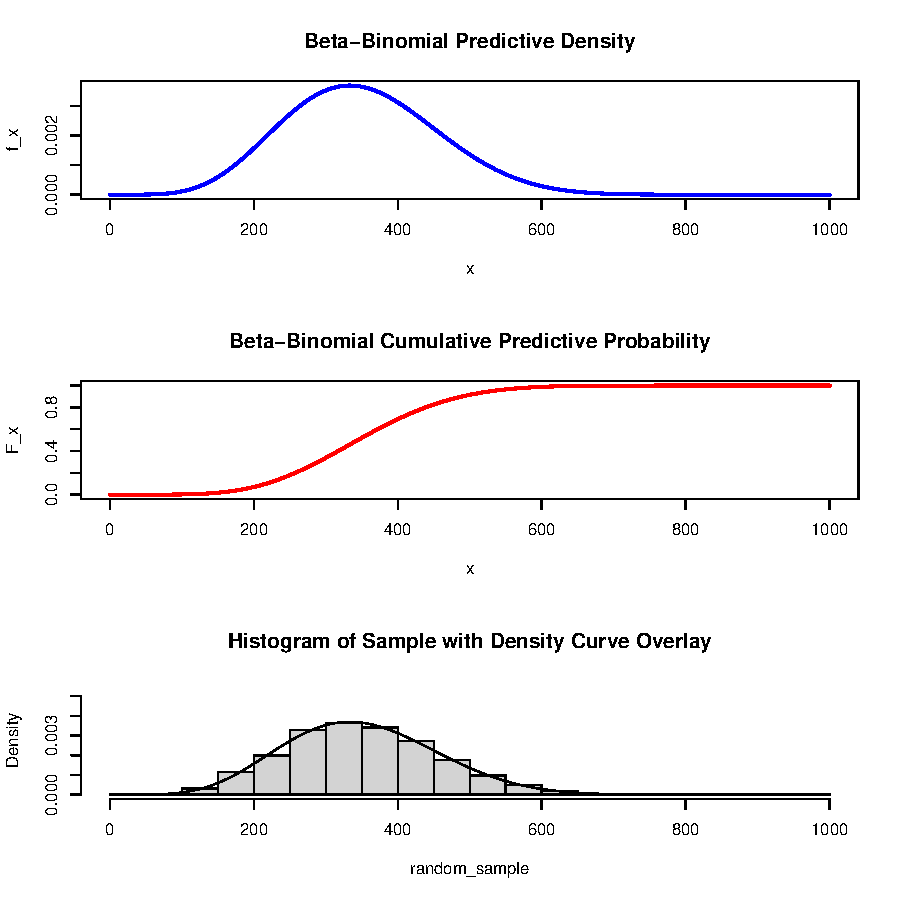
\includegraphics{Thesis-002}



    \subsection{Survival Time:  Exponential-Gamma (Geisser p. 74)}


    \subsubsection{Derivation}

      Suppose $X^{(N)} = \left(X^{(d)},X^{(N-d)}\right)$ where $X^{(d)}$ represents copies fully observed from an exponential survival time density
          $$f(x|\theta) = \theta e^{-\theta x}$$
      and $X^{(N-d)}$ represents copies censored at $x_{d+1},...,x_N$, respectively.  Hence
          $$L(\theta)\propto\theta^d e^{-\theta N\bar{x}}$$
      when $N\bar{x} = \sum_1^N{x_i}$, as shown below.\\

      The usual exponential likelihood is used for the fully observed copies, whereas for the censored copies we need Pr$(x > \theta) = 1 - \text{Pr}(x\leq\theta) = 1 - F(x|\theta) = 1 - (1 - e^{-\theta x}) = e^{-\theta x}$.  Thus the overall likelihood is

      $$L(\theta|x) = \prod_{i=1}^d\theta e^{-\theta x_i}\prod_{i=d+1}^N e^{-\theta x_i} = \theta^d e^{-\theta N\bar{x}}$$

      Assuming a Gamma$(\delta,\gamma)$ prior for $\theta$,

       $$p(\theta) = \frac{\gamma^\delta\theta^{\delta - 1}e^{-\gamma\theta}}{\Gamma(\delta)}$$

       we obtain the posterior

       %$$p\left(\theta|X^{(N)}\right) = \frac{p\left(x^{(N)}|\theta\right)p(\theta)}{\int p\left(X^{(N)}|\theta\right)p(\theta)d\theta} = \frac{(\gamma+N\bar{x})^{d+\delta}\theta^{d+\delta - 1}e^{-\theta(\gamma+N\bar{x})}}{\Gamma(d+\delta)}$$

        \begin{flalign*}
          p\left(\theta|X^{(N)}\right)
          &= \frac{p\left(x^{(N)}|\theta\right)p(\theta)}{\int p\left(X^{(N)}|\theta\right)p(\theta)d\theta}\\
          &\\
          &= \frac{\theta^d e^{-\theta N\bar{x}}\cdot\frac{\gamma^\delta\theta^{\delta - 1}e^{-\gamma\theta}}{\Gamma(\delta)}}{\int\left(\theta^d e^{-\theta N\bar{x}}\cdot\frac{\gamma^\delta\theta^{\delta - 1}e^{-\gamma\theta}}{\Gamma(\delta)}\right)d\theta}\\
          &\\
          &= \frac{\cancel{\frac{\gamma^\delta}{\Gamma(\delta)}}\left(\theta^{d+\delta - 1}e^{-\theta(\gamma+N\bar{x})}\right)}{\cancel{\frac{\gamma^\delta}{\Gamma(\delta)}}\int\left(\theta^{d+\delta - 1}e^{-\theta(\gamma+N\bar{x})}\right)d\theta}\\
          &\\
          &= \frac{\frac{(\gamma+N\bar{x})^{d+\delta}}{\Gamma(d+\delta)}\left(\theta^{d+\delta - 1}e^{-\theta(\gamma+N\bar{x})}\right)}{\cancel{\frac{(\gamma+N\bar{x})^{d+\delta}}{\Gamma(d+\delta)}\int\left(\theta^{d+\delta - 1}e^{-\theta(\gamma+N\bar{x})}\right)d\theta}}\\
          &\\
          &= \frac{(\gamma+N\bar{x})^{d+\delta}\theta^{d+\delta - 1}e^{-\theta(\gamma+N\bar{x})}}{\Gamma(d+\delta)}
        \end{flalign*}

    with the Gamma$(d+\delta,\gamma+N\bar{x})$ density in the next to last step integrating to $1$.\\

    Thus the survival time predictive probability is

    \begin{flalign*}
      P\left(X = x|\theta,X^{(N)}\right)
      &= \int p\left(\theta|X^{(N)}\right)p(x|\theta)d\theta\\
      &\\
      &= \int\frac{(\gamma+N\bar{x})^{d+\delta}\theta^{d+\delta - 1}e^{-\theta(\gamma+N\bar{x})}}{\Gamma(d+\delta)}\cdot\theta e^{-\theta x}d\theta\\
      &\\
      &= (d+\delta)(\gamma+N\bar{x})^{d+\delta}\int\frac{\theta^{(d+\delta + 1) - 1}e^{-\theta(\gamma+N\bar{x} + x)}}{(d+\delta)\Gamma(d+\delta)}d\theta\\
      &\\
      &= \frac{(d+\delta)(\gamma+N\bar{x})^{d+\delta}}{\left(\gamma+N\bar{x}+x\right)^{d+\delta+1}}\int\frac{\left(\gamma+N\bar{x}+x\right)^{d+\delta+1}\theta^{(d+\delta + 1) - 1}e^{-\theta(\gamma+N\bar{x} + x)}}{\Gamma(d+\delta+1)}d\theta\\
      &\\
      &= \frac{(d+\delta)(\gamma+N\bar{x})^{d+\delta}}{\left(\gamma+N\bar{x}+x\right)^{d+\delta+1}}
    \end{flalign*}

    (simplifying by constructing a Gamma$(d+\delta+1,\gamma+N\bar{x}+x)$ density in the final integrand.)\\



    \subsubsection{R Implementation}

This result has been used to create standard format R functions dpredEG(), ppredEG(), and rpredEG() for the Gamma-Exponential distribtuion for density, cumulative probability, and random sampling, respectively (see appendix).  These functions are exercised in the following example.


    \subsubsection{Example}

Suppose $d=800$ out of $N = 1000$ copies have been observed, and the remaining $200$ censored.  Say $\delta = 20$, $\gamma=5$, and we are interested in the number of survivors out of $M = 1000$ future observations.  The figures below illustrate the predictive probability using dpredEG() and rpredEG(), along with a histogram of a random sample taken using rpredEG().


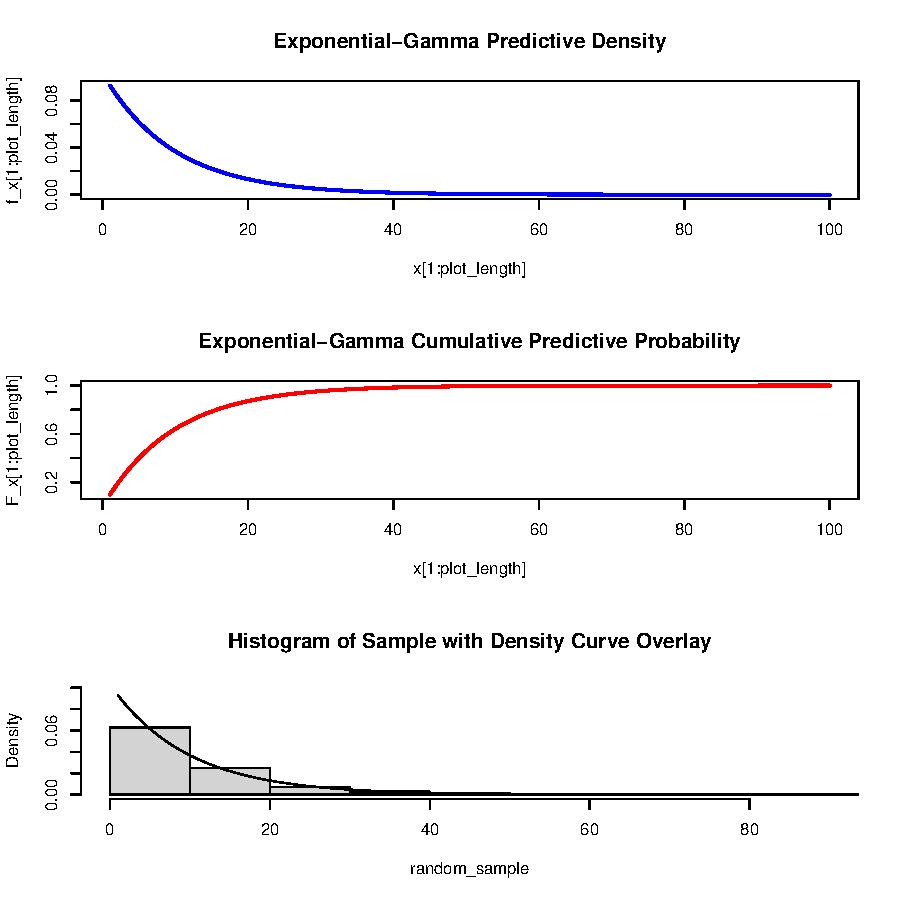
\includegraphics{Thesis-003}

\clearpage

  \subsection{Poisson-Gamma Model (Hoff p. 43ff)}
    \subsubsection{Derivation}
    [using Hoff's notation and variable names below.  Should I convert this to Geisser's $x^{(N)},x_{(M)}$ convention for uniformity throughout my thesis?]\\\\
      Suppose $Y_1,...,Y_n|\theta\overset{i.i.d.}{\sim}\text{Poisson}(\theta)$ with Gamma prior $\theta\sim\text{Gamma}(\alpha,\beta)$.  That is,

      \begin{flalign*}
        P\left(Y_1 = y_1,...,Y_n = y_n|\theta\right)
        &= \prod_{i=1}^n p\left(y_i|\theta\right)\\
        &\\
        &= \prod_{i=1}^n\frac{1}{y!}\theta^{y_i}e^{-\theta}\\
        &\\
        &= \left(\prod_{i=1}^n\frac{1}{y!}\right)\theta^{\sum y_i}e^{-n\theta}\\
        &\\
        &= c\left(y_1,...,y_n\right)\theta^{\sum y_i}e^{-n\theta}
      \end{flalign*}

      and

      $$p(\theta) = \dfrac{\beta^\alpha}{\Gamma(\alpha)}\theta^{\alpha-1}e^{-\beta\theta}, \theta, \alpha, \beta > 0.$$

\bigskip

      Then we have posterior distribution

      \begin{flalign*}
        p\left(\theta|y_1,...,y_n\right)
        &= \dfrac{p\left(y_1,...,y_n|\theta\right)p(\theta)}{\int_\theta p\left(y_1,...,y_n|\theta\right)p(\theta)}\\
        &\\
        &= \dfrac{p\left(y_1,...,y_n|\theta\right)p(\theta)}{p\left(y_1,...,y_n\right)}\\
        &\\
        &= \dfrac{1}{p\left(y_1,...,y_n\right)}\theta^{\sum y_i}e^{-n\theta}\dfrac{\beta^\alpha}{\Gamma(\alpha)}\theta^{\alpha - 1}e^{-\beta\theta}\\
        &\\
        &= C\left(y_1,...,y_n,\alpha,\beta\right)\theta^{\alpha+\sum y_i - 1}e^{-(\beta + n)\theta}\\
        &\\
        &\sim \text{Gamma}\left(\alpha+\sum y_i,\beta + n\right).
      \end{flalign*}


      Here

      \begin{flalign*}
        C\left(y_1,...,y_n,\alpha,\beta\right)
        &= \dfrac{1}{p\left(y_1,...,y_n\right)}\cdot\dfrac{\beta^\alpha}{\Gamma(\alpha)}\\
        &\\
        &= \dfrac{1}{\int_\theta p\left(y_1,...,y_n|\theta\right)p(\theta)}\cdot\dfrac{\beta^\alpha}{\Gamma(\alpha)}\\
        &\\
        &= \dfrac{1}{\int_\theta\left(\prod\frac{1}{y_i!}\right)\theta^{\sum y_i}e^{-n\theta}\cancel{\left(\frac{\beta^\alpha}{\Gamma(\alpha)}\right)}\theta^{\alpha-1}e^{-\beta\theta}}\cdot\cancel{\left(\frac{\beta^\alpha}{\Gamma(\alpha)}\right)}
        &\\
        &= \dfrac{1}{\left(\prod\frac{1}{y_i!}\right)\frac{\Gamma(\alpha + \sum y_i)}{(\beta+n)^{\alpha+\sum y_i}}\int_\theta \frac{(\beta+n)^{\alpha+\sum y_i}}{\Gamma(\alpha+\sum y_i)}\theta^{\sum y_i+\alpha-1}e^{-(\beta+n)\theta}}\\
        &\\
        &= \dfrac{\prod_{i=1}^n y_i!(\beta+n)^{\alpha+\sum y_i}}{\Gamma(\alpha+\sum y_i)}
      \end{flalign*}

      Call this constant $C_n$ (for $n$ observations).

\bigskip

      Note that an additional observation $y_{n+1} = \tilde{y}$ the constant becomes

      $$C_{n+1} = \dfrac{\prod_{i=1}^{n+1} y_i!(\beta+n+1)^{\alpha+\sum_{i=1}^{n+1} y_i}}{\Gamma(\alpha+\sum_{i=1}^{n+1} y_i)}.$$

      Also note that the marginal joint distribution of $k$ observations is

      $$p\left(\tilde{y}|y_1,...,y_k\right) = \dfrac{1}{C_k}\dfrac{\beta^\alpha}{\Gamma(\alpha)}.$$

      For future observation $\tilde{y}$, then, we compute predictive distribution

      \begin{flalign*}
        p\left(\tilde{y}|y_1,...,y_n\right)
        &= \dfrac{p\left(y_1,...,y_n,\tilde{y}\right)}{p\left(y_1,...,y_n\right)} = \dfrac{p\left(y_1,...,y_{n+1}\right)}{p\left(y_1,...,y_n\right)}
        = \dfrac{\frac{1}{C_{n+1}}\cancel{\frac{\beta^\alpha}{\Gamma(\alpha)}}}{\frac{1}{C_n}\cancel{\frac{\beta^\alpha}{\Gamma(\alpha)}}}
        = \dfrac{C_n}{C_{n+1}}\\
        &\\
        &= \dfrac{\dfrac{\prod_{i=1}^n y_i!(\beta+n)^{\alpha+\sum_{i=1}^n y_i}}{\Gamma(\alpha+\sum_{i=1}^n y_i)}}{\dfrac{\prod_{i=1}^{n+1} y_i!(\beta+n+1)^{\alpha+\sum_{i=1}^{n+1} y_i}}{\Gamma(\alpha+\sum_{i=1}^{n+1} y_i)}}\\
        &\\
        &= \dfrac{\Gamma\left(\alpha+\sum_{i=1}^{n+1}y_i\right)(\beta+n)^{\alpha+\sum_{i=1}^n y_i}}{\left(y_{n+1}!\right)\Gamma\left(\alpha+\sum_{i=1}^n y_i\right)(\beta+n+1)^{\alpha+\sum_{i=1}^{n+1}y_i}}\\
        &\\
        &= \dfrac{\Gamma\left(\alpha+\sum_{i=1}^n y_i + \tilde{y}\right)(\beta+n)^{\alpha+\sum_{i=1}^n y_i}}{\left(\tilde{y}!\right)\Gamma\left(\alpha+\sum_{i=1}^n y_i\right)(\beta+n+1)^{\alpha+\sum_{i=1}^n y_i + \tilde{y}}}\\
        &\\
        &= \dfrac{\Gamma\left(\alpha+\sum y_i+\tilde{y}\right)}{\Gamma(\tilde{y}+1)\Gamma(\alpha+\sum y_i)}\cdot \left(\dfrac{\beta+n}{\beta+n+1}\right)^{\alpha+\sum y_i} \cdot \left(\dfrac{1}{\beta+n+1}\right)^{\tilde{y}}\\
      \end{flalign*}

This is a negative binomial distribution:  $\tilde{y}\sim NB\left(\alpha+\sum y_i,\beta+n\right)$.

\vspace{5mm}

\hrule

\vspace{5mm}

$$\theta\sim NB(\alpha,\beta)\Rightarrow p(\theta) = \binom{\theta+\alpha-1}{\alpha - 1}\left(\dfrac{\beta}{\beta+1}\right)^\alpha\left(\dfrac{1}{\beta+1}\right)^\theta$$

\begin{center}so\end{center}

\begin{flalign*}
  \tilde{y}\sim NB\left(\alpha + \sum{y_i}),\beta+n\right)\Rightarrow p(\tilde{y})
  &= \binom{\tilde{y}+\alpha+\sum{y_i}-1}{\alpha+\sum{y_i}-1}\left(\dfrac{\beta+n}{\beta+n+1}\right)^{\alpha+\sum{y_i}}\left(\dfrac{1}{\beta+n+1}\right)^{\tilde{y}}\\
  &\\
  &= \dfrac{\left(\alpha + \sum{y_i} + \tilde{y} - 1\right)!}{\left(\alpha + \sum{y_i} - 1\right)!\left(\tilde{y}\right)!}\left(\dfrac{\beta+n}{\beta+n+1}\right)^{\alpha+\sum{y_i}}\left(\dfrac{1}{\beta+n+1}\right)^{\tilde{y}}\\
  &\\
  &= \dfrac{\Gamma\left(\alpha + \sum{y_i} + \tilde{y}\right)}{\Gamma\left(\alpha + \sum{y_i}\right)\Gamma\left(\tilde{y}+1\right)}\left(\dfrac{\beta+n}{\beta+n+1}\right)^{\alpha+\sum{y_i}}\left(\dfrac{1}{\beta+n+1}\right)^{\tilde{y}}
\end{flalign*}

\vspace{5mm}

\hrule

\vspace{5mm}

      \bigskip



      [This is the result in Hoff.  The straightforward derivation below is off by a constant multiple.  Need to figure out what went awry.]



      \begin{flalign*}
        p\left(\tilde{y}|y_1,...,y_n\right)
        &= \int_0^\infty p\left(\tilde{y}|\theta,y_1,...,y_n\right)p\left(\theta|y_1,...,y_n\right)d\theta\\
        &\\
        &= \int p\left(\tilde{y}|\theta\right)p\left(\theta|y_1,...,y_n\right)d\theta\\
        &\\
        &= C\int\left(\dfrac{1}{\tilde{y}!}\theta^{\tilde{y}}e^{-\theta}\right)\theta^{\alpha+\sum y_i - 1}e^{-(\beta+n)\theta}d\theta\\
        &\\
        &= \dfrac{C}{\tilde{y}!}\int\theta^{\tilde{y}+\alpha+\sum y_i - 1}e^{-(\beta+n+1)\theta}d\theta\\
        &\\
        &= \dfrac{C\Gamma\left(\tilde{y}+\alpha+\sum y_i\right)}{\Gamma\left(\tilde{y}+1\right)(\beta+n+1)^{\tilde{y}+\alpha+\sum y_i}}\int\dfrac{(\beta+n+1)^{\tilde{y}+\alpha+\sum y_i}}{\Gamma\left(\tilde{y}+\alpha+\sum y_i\right)}\theta^{\tilde{y}+\alpha+\sum y_i - 1}e^{-(\beta+n+1)\theta)}d\theta\\
        &\\
        &= C\cdot\dfrac{\Gamma\left(\tilde{y}+\alpha+\sum y_i\right)}{\Gamma\left(\tilde{y}+1\right)(\beta+n+1)^{\tilde{y}+\alpha+\sum y_i}}\\
        &\\
        &= \dfrac{\prod_{i=1}^n y_i!(\beta+n)^{\alpha+\sum y_i}}{\Gamma(\alpha+\sum y_i)}\cdot\dfrac{\Gamma\left(\tilde{y}+\alpha+\sum y_i\right)}{\Gamma\left(\tilde{y}+1\right)(\beta+n+1)^{\tilde{y}+\alpha+\sum y_i}}\\
        &\\
        &= \prod_{i=1}^n y_i! \cdot \dfrac{\Gamma\left(\tilde{y}+\alpha+\sum y_i\right)}{\Gamma(\tilde{y}+1)\Gamma(\alpha+\sum y_i)}\cdot \left(\dfrac{\beta+n}{\beta+n+1}\right)^{\alpha+\sum y_i} \cdot \left(\dfrac{1}{\beta+n+1}\right)^{\tilde{y}}\\
      \end{flalign*}

\textcolor{red}{Hoff p.47:
  \begin{itemize}
    \item $b$ is interpreted as the number of prior observations
    \item $a$ is interpreted as the sum of counts from $b$ prior observations
  \end{itemize}
}

\textcolor{red}{  Hoff p. 49 (Birth rate example):  $a = 2, b = 1$. }


    \subsubsection{R Implementation}

This result has been used to create standard format R functions dpredPG(), ppredPG(), and rpredPG() for the Poisson-Gamma distribtuion for density, cumulative probability, and random sampling, respectively (see appendix).  These functions are exercised in the following example.

    \subsubsection{Example}

Suppose $t=5$ successes have been observed out of $N=10$ binary events, $\alpha = 2$ and $\beta = 8$.  For $M = 1000$ future observations, the figures below show the predictive distribution from dpredBB(), the cumulative distribution from ppredBB(), and a histogram of random draws from rpredBB().

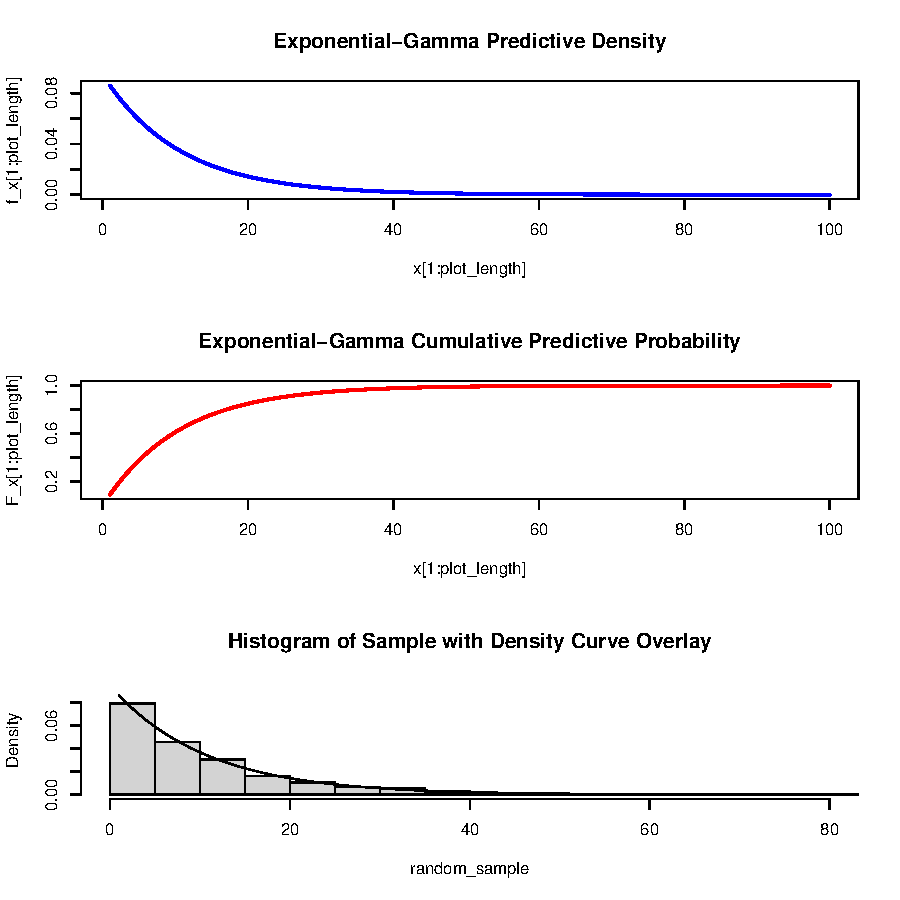
\includegraphics{Thesis-004}


  \subsection{Normal Observation with Normal-Inverse Gamma Prior}
    \subsubsection{One sample}
      \paragraph{Derivation}
      \paragraph{R Implementation}
      \paragraph{Example}
    \subsubsection{Two samples}
      \paragraph{Derivation}
      \paragraph{R Implementation}
      \paragraph{Example}
    \subsubsection{$k$ samples}
      \paragraph{Derivation}
      \paragraph{R Implementation}
      \paragraph{Example}
      \paragraph{Ranking Treatments}

\clearpage


\section{Chapter 2:  Normal Regression with Zellner's $g$-prior}
  \paragraph{Derivation}
  \paragraph{R Implementation}
  \paragraph{Example}


\clearpage

\section{Conclusion}

\end{document}
